\documentclass{standalone}

\usepackage{tikz}

\usetikzlibrary{positioning, chains, shapes.geometric, fit, shapes, arrows.meta, calc}

\begin{document}

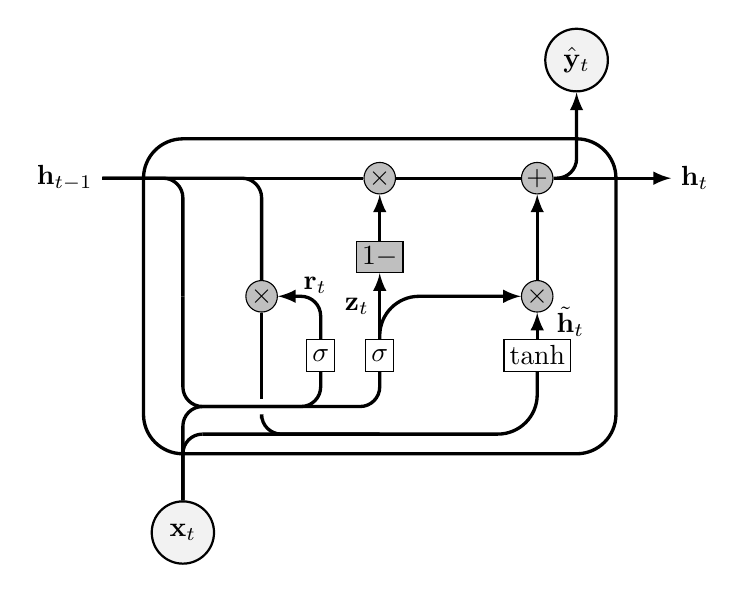
\begin{tikzpicture}[
    >=LaTeX, % Use default LaTeX arrows
    % Styles 
    cell/.style={ % RNN cell
        rectangle, 
        rounded corners=5mm, 
        draw,
        very thick,
        minimum height=4cm,
        minimum width=6cm
    }, 
    cellc/.style={ % RNN cells in a chain
        cell,
        on chain,
        join
    },
    input/.style={ % Input or output node
        circle,
        minimum width=2.25em,
        draw,
        fill=gray!10,
        thick
    },
    hidden/.style={ % Hidden state
    },
    func/.style={ % Functions
        rectangle,
        draw,
        inner sep=2pt,
        minimum height=0.4cm
    },
    op/.style={ % Operators
        circle,
        draw,
        inner sep=-0.5pt,
        minimum height=0.4cm,
    },
    pointwise/.style={ % Pointwise operations and functions
        fill=gray!50,
    },
    arrow/.style={
        -latex,
        very thick
    },
    arrowc1/.style={ % Arrows with rounded corners
        arrow,
        rounded corners=.25cm
    },
    arrowc2/.style={ % Arrows with big rounded corners
        arrow,
        rounded corners=.5cm
    },
    backprop/.style={ % Backpropagation arrows
        arrow,
        dashed,
        gray
    }
]
  
    % GRU cell
    \node [cell] at (0,0){};

    % Internal functions and operators
    \node [func] (sigr) at (-0.75,-0.75) {$\sigma$};
    \node [func] (sigz) at (0,-0.75) {$\sigma$};
    \node [func] (tanh) at (2,-0.75) {$\tanh$};
    \node [func, pointwise] (minus) at (0,0.5) {$1-$};
    \node [op, pointwise] (mulr) at (-1.5,0) {$\times$};
    \node [op, pointwise] (mulz) at (0,1.5) {$\times$};
    \node [op, pointwise] (add) at (2,1.5) {$+$};
    \node [op, pointwise] (mulh) at (2,0) {$\times$};

    % Inputs, outputs and hidden states
    \node[hidden] (ht-1) at (-4,1.5) {$\mathbf{h}_{t-1}$};
    \node[input] (x) at (-2.5,-3) {$\mathbf{x}_{t}$};
    \node[hidden] (ht) at (4,1.5) {$\mathbf{h}_{t}$};
    \node[input] (y) at (2.5,3) {$\hat{\mathbf{y}}_{t}$};

    % Arrows from input and previous hidden states h_{t-1}
    \draw [arrowc1] (ht-1) -- (mulz) -- (add) -- (ht);
    \draw [arrowc1, -] (x) |- (-2.25, -1.4) ++(sigr);
    \draw [arrowc1, -] (x) |- (-2.25, -1.75) ++(sigr);
    \draw [arrowc1, -] (x -| sigz) ++(-1, 1.6) -| (sigz);
    \draw [arrowc1, -] (x -| sigr) ++(-1.5, 1.6) -| (sigr);
    \draw [arrowc1, -] (ht-1.east) -| (mulr);
    \draw [arrowc1, -] (ht-1) -| (-2.5,0) ++(x);
    \draw [arrowc1, -] (x) ++(0,3) |- (-1,-1.4) ++(tanh);
    \draw [arrowc2, -] (x -| tanh) ++(-4.25, 1.25) -| (tanh);

    % Arrows for operation flow within LSTM gates
    \draw [arrowc1, -] (mulr) -- ++(0,-1.3);
    \draw [arrowc1, -] (mulr) ++(0,-1.55) |- (0,-1.75) ++(tanh);
    \draw [arrowc1] (sigr) |-  node[midway, shift={(-2pt,4pt)}] {$\mathbf{r}_t$} (mulr.east);
    \draw [arrowc2] (sigz) |- (mulh);
    \draw [arrowc2] (tanh) -- node[midway, shift={(12pt,1.5pt)}] {$\tilde{\mathbf{h}}_t$} (mulh);
    \draw [arrowc2] (minus) -- (mulz);
    \draw [arrowc2] (sigz) -- node[midway, left] {$\mathbf{z}_t$} (minus);
    \draw [arrowc2] (mulh) -- (add);

    % Arrows to output and current hidden states h_t
    \draw [arrowc1] (add) coordinate[auto] -|(y);
\end{tikzpicture}

\end{document}